% Documento principal del informe de la Entrega 1.
% Máximo 6 páginas de cuerpo; la portada y los anexos no cuentan.
% Cada sección vive en su propio .tex para que cada responsable edite la suya.
\documentclass[11pt,a4paper]{article}
\usepackage[utf8]{inputenc}
\usepackage[T1]{fontenc}
\usepackage{lmodern}
\usepackage[spanish]{babel}
\usepackage[margin=2.5cm]{geometry}
\usepackage{graphicx}
\usepackage{booktabs}
\usepackage{array}
\usepackage{longtable}
\usepackage[hidelinks]{hyperref}
\usepackage[font=small,skip=3pt]{caption}
% El cuerpo tiene más de veinte \paragraph; el espacio por defecto antes de cada uno
% (3,25ex) suma casi un cuarto de página. Se aprieta a 1,6ex, que sigue separando bien.
\usepackage{titlesec}
\titlespacing*{\paragraph}{0pt}{1.6ex plus .4ex minus .2ex}{1em}
\setlength{\textfloatsep}{8pt plus 2pt minus 2pt}
\setlength{\intextsep}{8pt plus 2pt minus 2pt}
% figuras/ en Overleaf; ../output/figuras/ al compilar en local desde informe/
\graphicspath{{figuras/}{../output/figuras/}}

% Todas las cifras del informe quedaron verificadas contra output/cifras.md (componente B),
% así que la marca de «por confirmar» está apagada.
\newcommand{\porconfirmar}[1]{#1}

\begin{document}

\begin{titlepage}
  \centering
  {\large IIC3752 Tecnologías para Inteligencia de Negocios\par}
  {\large Escuela de Ingeniería UC - 2026-2\par}
  \vspace{4cm}
  {\LARGE\bfseries Entrega 1\par}
  \vspace{0.5cm}
  {\Large Viña Vallehondo - Grupo 2\par}
  \vspace{3cm}
  {\large Integrantes\par}
  \vspace{0.3cm}
  [Diego Da Silva]\par
  [Nicolás Massa]\par
  [Nombre completo 3]\par
  [Benjamín Suazo]\par
  \vfill
  Repositorio: \url{https://github.com/Benjaa7/vina-g2}\par
  \vspace{0.5cm}
  14 de octubre de 2026
\end{titlepage}

% Sección A · Mandato acordado. Máximo 1 página (lo exige el enunciado).
% Requiere en el preámbulo: booktabs, array (los mismos de la sección C).
%
% CIFRAS: todas las de esta sección vienen de la exploración de septiembre y
% deben confirmarse contra output/cifras.md (componente B) antes de entregar:
%   11,2 % · 4,574 y 5,085 USD/L · 0,15–0,19 % de baja en listas
%   3,82 % y 4,40 % de descuento · 22,7 % y 32,5 % de mezcla
%   USD 77,26 y 77,20 por caja · 4,47 / 4,83 / 5,03 USD/L
% Van marcadas solo las dos de titular, para no romper la lectura.
\providecommand{\porconfirmar}[1]{\textbf{#1}\,[por confirmar]}

\section{Mandato acordado}

Cada hallazgo va marcado con su origen: \textbf{(V)} verbalizado por la contraparte, \textbf{(M)} medido por nuestro análisis, \textbf{(I)} inferido por el equipo.

\paragraph{La pregunta.} De las cuatro del README, trabajamos la segunda: el precio promedio por litro que subió, ¿es porque subimos precios o porque vendimos mayor proporción de gran reserva?

\paragraph{Por qué esa.} La elección sale de la reunión del 4 de septiembre. Sin que se lo preguntáramos, la contraparte identificó el origen del encargo: «tenemos este problema de la conversión entre cajas y litros, porque no todas las cajas tienen el mismo número de litros; nos dimos cuenta que teníamos un problema y por eso los llamamos» (V). Nombró el vacío que quiere cerrar, «no se disgrega cepa, reserva, gran reserva ni varietal al tomar la decisión» (V), y declaró que su unidad de medida es el litro (V): de ahí que midamos por litro y no por caja.

El dato confirma que la pregunta no es obvia. Entre el primer y el segundo semestre de 2025 el precio medio por litro de exportación subió \porconfirmar{11,2 \%}, de 4,574 a 5,085 USD/L, mientras los precios de lista bajaron entre 0,15 \% y 0,19 \% en los tres tiers y el descuento medio subió de 3,82 \% a 4,40 \% (M). La participación de gran reserva pasó de 22,7 \% a 32,5 \% de los litros (M). Si el precio efectivo sube mientras las listas bajan, el alza es de mezcla, no de precio (I).

\paragraph{Por qué no las otras.} La primera, sobre el tipo de cambio, se usa como contexto: la contraparte no lo mencionó como problema en toda la reunión y declaró no tener política formal para valorizar exportaciones (V), así que no hay cita que la justifique. La tercera, sobre margen por mercado, no es respondible con lo entregado: la contraparte señaló que faltan los aranceles por tratado de libre comercio, los costos de despacho y el tramo de dólar a euro de los clientes europeos (V); sin ellos, CIF y FOB rinden el mismo margen en nuestros datos, lo que es falso (M). La cuarta, sobre qué fecha usar para convertir, queda como definición secundaria: la contraparte cerró que el año «se cierra por factura, no por despacho» (V), y adoptamos la fecha de factura por consistencia (I).

\paragraph{El hilo de correo.} El hilo se abrió el 8 de septiembre con el acta, donde quedó comprometido confirmar por esa vía la equivalencia de caja a litro. La contraparte ofreció enviar los aranceles por país, los costos de despacho y la información financiera (V).
% ---------------------------------------------------------------------------
% ELEGIR UNA DE LAS DOS FRASES SIGUIENTES Y BORRAR LA OTRA.
%
% (1) Si NO se enviaron las consultas dentro del plazo o no se aceptaron:
No se alcanzó a realizar ninguna consulta dentro del plazo, de modo que la equivalencia de caja a litro, el tratamiento del monto neto y la estacionalidad del alza quedan cerrados como supuestos del equipo (bitácora S1, S3 y S8).
%
% (2) Si sí respondieron, reemplazar por algo de esta forma:
% La contraparte respondió el [fecha] que [lo que dijo, textual] (V), con lo que la definición de caja a litro queda [confirmada / corregida a X litros].
% ---------------------------------------------------------------------------

\paragraph{La definición que la contraparte no cerró.} Es la equivalencia entre caja y litro según el formato, que sostiene toda la métrica. Operaciones afirmó que «no todas las cajas tienen el mismo número de litros» (V). El maestro de costos declara 9,0 litros por caja para los dos únicos formatos, 12$\times$750 y 6$\times$1500 (M), que por aritmética dan 9 litros exactos. Y el precio medio por caja del magnum, USD 77,26, coincide con el del gran reserva estándar, USD 77,20 (M), lo que solo se sostiene si ambos rinden los mismos litros (I).

Ante la contradicción, la cerramos en 9,0 litros por caja para ambos formatos. El criterio: cuando lo que dice el cliente y lo que muestra el dato no coinciden, adoptamos el dato si existe una verificación independiente de él. Aquí la hay, y viene de otro archivo: los litros salen del maestro de costos y el precio por caja de la base de ventas. Queda en la bitácora (S1) con su efecto: si el magnum no rindiera 9 litros, el precio medio se movería entre \porconfirmar{4,47 y 5,03 USD/L} frente a los 4,83 adoptados (M); la sensibilidad completa va en la sección D.

% Sección B · Cadena ejecutable. Extensión sugerida: 0,5 página en el informe; el resto es el repositorio.


\section{Cadena ejecutable}

La cadena lee las cuatro fuentes del caso, las limpia, construye el modelo de la sección~3 y calcula todas las cifras y figuras del informe. Se ejecuta con un solo comando desde la carpeta \texttt{E1} del repositorio:

\begin{center}
\texttt{pip install -r requirements.txt} \quad y luego \quad \texttt{python run.py}
\end{center}

\noindent Corre en Python 3.11 o superior y demora entre 7 y 35 segundos, según lo que tarde la API. El README del repositorio detalla la instalación y las cifras que deben aparecer al final.

\paragraph{Flujo.} Cuatro etapas, cada una en su módulo: \emph{extraer} (lee las fuentes) $\rightarrow$ \emph{limpiar} (aplica las reglas de calidad y cuenta las filas que toca cada una) $\rightarrow$ \emph{integrar} (construye \texttt{fact\_venta} y sus dimensiones) $\rightarrow$ \emph{métrica} (indicador, descomposición, sensibilidades y figuras). Ninguna cifra del informe está escrita a mano: todas salen de \texttt{output/cifras.md}, que la cadena regenera en cada ejecución.

\paragraph{Qué aporta cada fuente:}La pregunta se apoya sobre todo en ventas y costos, pero las cuatro fuentes entran al proceso con un rol concreto:

\texttt{origen\_vina.sqlite} aporta las líneas de venta (13.845 tras deduplicar) y las tablas de clientes, mercados, zonas, cepas y monedas que forman las dimensiones. \texttt{origen\_costos\_productos.csv} aporta los litros y el costo por caja de cada producto y añada, y sostiene la conversión de caja a litro. \texttt{origen\_embarques.json} corrige las líneas cargadas en botellas en vez de cajas e identifica el incoterm, pero no se usa para fecha ni mercado: el 64\,\% de sus líneas declara un mercado distinto al de la venta. La API \texttt{mindicador.cl} aporta el dólar observado diario de 2025 y 2026, para expresar los montos en pesos.

\paragraph{Reglas de limpieza.} La cadena no corrige las fuentes: las lee como vienen y aplica reglas explícitas, cada una registrada con su conteo en \texttt{output/cobertura.md} y detallada en el anexo~B.

\paragraph{Reproducibilidad.} Se probó en dos ambientes limpios (Python 3.12 y 3.14), clonando el repositorio y siguiendo solo el README: las salidas son idénticas byte a byte. Si la API no responde, usa la copia guardada de la serie y lo avisa, con el mismo resultado; en la última prueba la API estaba caída y corrió igual. Si una regla encuentra un caso que no sabe tratar, la ejecución se detiene con un error en vez de seguir en silencio.

\paragraph{Qué se espera ver al final.} Al terminar, \texttt{run.py} imprime seis cifras de verificación: las 13.845 filas de \texttt{fact\_venta}, las 10.672 del universo de la métrica, la participación de gran reserva (22,7\,\% $\rightarrow$ 32,5\,\%), el precio medio por litro (4,574 $\rightarrow$ 5,085 USD/L), el precio medio anual (4,83 USD/L) y el peso del magnum (8,07\,\% del volumen y 13,76\,\% del ingreso). Las mismas, con todas las demás del informe, quedan en \texttt{output/cifras.md} con su definición y el lugar donde aparecen.

% Sección C · Modelo dimensional. Requiere en el preámbulo: graphicx, booktabs, array.
% \porconfirmar marca las cifras que deben salir de output/cifras.md (componente B).
% Cuando estén confirmadas, cambiar la definición por: \renewcommand{\porconfirmar}[1]{#1}
\providecommand{\porconfirmar}[1]{\textbf{#1}\,[por confirmar]}

\section{Modelo dimensional}

Modelamos un solo proceso de negocio, la venta: cada vez que se factura una línea de vino. Es una tabla de hechos transaccional con cuatro dimensiones a un salto (figura~\ref{fig:modelo}). La fuente viene normalizada en tablas encadenadas (ventas, mercados, zonas); la aplanamos en una estrella porque país y zona son niveles de una misma jerarquía.

\begin{quote}
\textbf{Grano.} Una fila es una línea de venta facturada: un producto de una añada, vendido a un cliente en una fecha.
\end{quote}

\begin{figure}[ht]
  \centering
  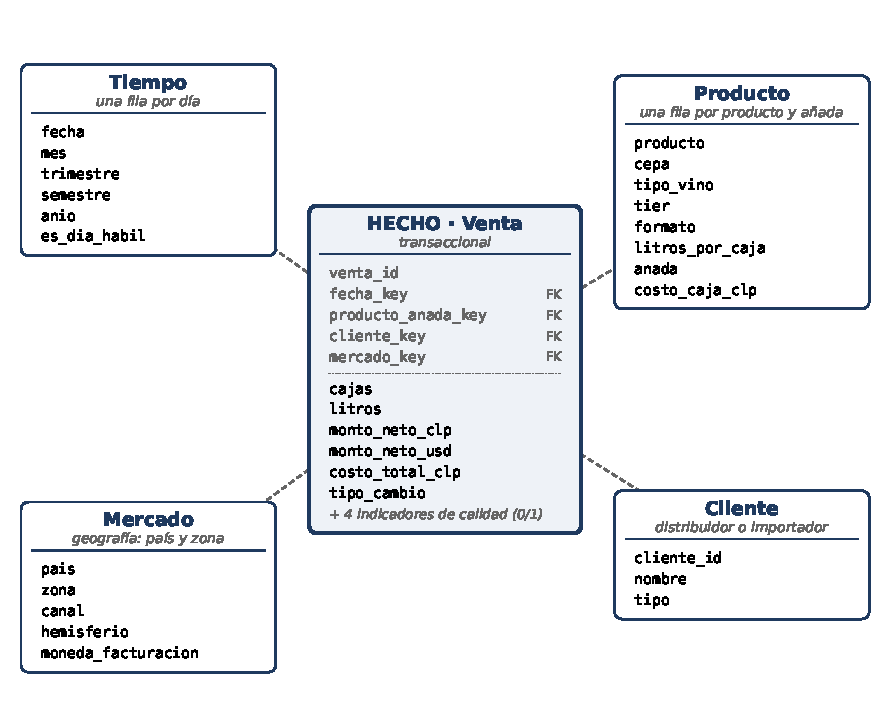
\includegraphics[width=0.66\textwidth]{modelo_estrella.pdf}
  \caption{Modelo estrella de la venta. Fuente: elaboración propia a partir de las cuatro fuentes del caso. Diccionario de datos en el anexo C.}
  \label{fig:modelo}
\end{figure}

Toda cifra del informe se calcula sumando filas de \texttt{fact\_venta}; ninguna sale de una tabla preagregada. De sus \porconfirmar{13.845} filas, \porconfirmar{10.672} son exportaciones de 2025 y forman el universo de la métrica (sección D).

\paragraph{Por qué este grano.} No existe en la fuente un nivel más fino que la línea de venta, y uno más grueso destruye la pregunta: para separar el efecto precio del efecto mezcla, cada fila tiene que conservar su tier y sus litros. Si agregáramos, por ejemplo, por mes y mercado, la mezcla quedaría fija dentro de cada agregado.

\paragraph{El precio por litro no se guarda.} El hecho guarda cajas, litros y montos, que se suman. El precio medio por litro es un indicador, la suma del monto neto dividida por la suma de los litros, y una razón de sumas no es aditiva: se calcula en cada corte, nunca se promedia. Esta decisión es también la respuesta de negocio: como es una razón, el precio por litro sube cuando crece la proporción de litros de los tiers caros, aunque no se mueva ningún precio de lista.

\paragraph{Producto al nivel de producto y añada.} El costo por caja depende del tier y de la añada, así que \texttt{dim\_producto} tiene una fila por producto y añada (\porconfirmar{96}): el costo unitario es atributo de la dimensión y el costo total es hecho. Ahí vive también \texttt{litros\_por\_caja}, de modo que la definición de caja a litro (sección D) es una sola columna y su sensibilidad se calcula cambiando ese atributo. La cepa, escrita con alias distintos en el archivo de costos, se conforma al catálogo de cepas del ERP.

\paragraph{Montos en dos monedas.} La exportación se factura en dólares y el mercado nacional en pesos. Para no sumar pesos con dólares, cada monto se guarda en dos columnas, convertidas con el dólar observado de la fecha de factura. La moneda no va como texto en el hecho: la determina el mercado, así que es atributo de \texttt{dim\_mercado}.

\paragraph{Qué quedó fuera.}

\begin{center}
\small
\begin{tabular}{@{}>{\raggedright\arraybackslash}p{0.24\textwidth}>{\raggedright\arraybackslash}p{0.68\textwidth}@{}}
\toprule
Qué & Por qué \\
\midrule
Embarque (JSON) & Es otro proceso, con su propio grano (un embarque agrupa varias líneas), y su vínculo con la venta no es confiable. La cadena lo usa para corregir cajas cargadas en botellas; queda como la siguiente estrella (anexo C). \\
Vendedor & Redundante: los cinco vendedores corresponden uno a uno a las cinco zonas. \\
RUT del cliente & No aporta a la pregunta; minimización de datos personales. \\
Flete, seguro, aranceles & No están en ninguna fuente. \\
Cobranza & Otro proceso, sin fechas de pago. \\
\bottomrule
\end{tabular}
\end{center}

\paragraph{Qué resuelve y qué no.} El modelo separa precio de mezcla, convierte sin mezclar monedas y costea según la añada. No resuelve el margen por mercado (faltan flete y aranceles), el efecto cambiario real (cobranza a 60 y 90 días, pago en euros) ni si el alza de la gran reserva es estacional: con un año de datos permite el corte mensual, pero no comparar un año con otro.

% Sección D · Métrica y sensibilidad.
% El desarrollo (datos de entrada, cálculo tier por tier, métodos alternativos y
% las otras tres decisiones) está en el anexo D, para respetar el límite de 6 páginas.

\section{Métrica y sensibilidad}

\paragraph{Qué medimos.} La métrica es el precio medio por litro de exportación de cada semestre de 2025:
\[
P = \frac{\sum_i M_i}{\sum_i L_i}, \qquad L_i = C_i \times k_i,
\]
donde, para cada línea de venta $i$, $M_i$ es el monto neto en USD (después de descuento), $L_i$ son los litros vendidos, $C_i$ son las cajas y $k_i$ son los litros por caja de su producto. La suma recorre las líneas de \texttt{fact\_venta} del canal exportación con fecha de factura en el semestre (10.672 en el año), incluidas las de merma, con signo negativo. Unidad: USD por litro. Es una razón de sumas, no un promedio de los precios de cada línea.

Entre el 1.\textsuperscript{er} y el 2.\textsuperscript{o} semestre, $P$ subió de 4,574 a 5,085 USD/L: +0,511 USD/L, un 11,2\,\%.

\paragraph{Por qué no basta con mirar $P$.} Un precio medio puede subir por dos razones distintas: porque cada vino se vende más caro (\emph{efecto precio}) o porque, con los mismos precios, se vende una mayor proporción del vino caro (\emph{efecto mezcla}). Para separarlas aplicamos la descomposición estándar de variación precio-mezcla (Kitagawa, 1955; Horngren, Datar y Rajan, \emph{Cost Accounting}). Para cada tier $t$, con $w_t$ su proporción de los litros y $p_t$ su precio por litro, el cambio de $P$ se reparte en tres términos que suman exactamente el alza: mezcla $\sum_t (w_{t,2}-w_{t,1})\,p_{t,1}$, precio $\sum_t w_{t,1}\,(p_{t,2}-p_{t,1})$ y cruzado $\sum_t (w_{t,2}-w_{t,1})(p_{t,2}-p_{t,1})$. El cálculo tier por tier está en el anexo~D. El criterio lo fijamos antes de mirar los resultados: el alza es de mezcla si ese efecto explica más de la mitad del cambio bajo todos los métodos y todas las definiciones alternativas. No usamos pruebas de significancia porque los datos no son una muestra sino todas las ventas del año: la incertidumbre no viene del azar sino de nuestras definiciones, y eso es lo que miden las sensibilidades.

\paragraph{Resultado.}

\begin{center}
\small
\begin{tabular}{l r r}
\hline
\textbf{Efecto} & \textbf{USD/L} & \textbf{\% del alza} \\
\hline
Mezcla & +0,551 & +108\,\% \\
Precio & $-$0,035 & $-$7\,\% \\
Cruzado & $-$0,005 & $-$1\,\% \\
\hline
\textbf{Cambio total} & \textbf{+0,511} & \textbf{100\,\%} \\
\hline
\end{tabular}
\end{center}

\noindent Vender 9,8 puntos más de gran reserva, el tier más caro, suma 0,81 USD/L al precio medio; vender 9,3 puntos menos de varietal resta 0,23. El efecto precio es negativo en los tres tiers: ninguno subió su precio por litro, porque los precios de lista bajaron entre 0,15\,\% y 0,19\,\% y el descuento medio subió de 3,82\,\% a 4,40\,\% (ambos ponderados por cajas). El término cruzado es apenas el 1\,\% del alza, así que la repartición no es ambigua. Según el criterio fijado, \textbf{el alza es de mezcla}.

\paragraph{La decisión de definición: cuántos litros tiene una caja.} El denominador son los litros, $L_i = C_i \times k_i$, así que el resultado depende de $k_i$. Aquí había una contradicción que tuvimos que cerrar. La contraparte afirmó que «no todas las cajas tienen el mismo número de litros» (V), pero el maestro de costos declara 9,0 litros para los dos formatos que vende la viña, la caja estándar de 12 botellas de 750\,ml y la magnum de 6 botellas de 1,5\,L (M). Además el precio y el costo por caja del magnum coinciden con los del gran reserva estándar (M), algo que solo tiene sentido si ambas cajas rinden lo mismo (I). Adoptamos $k_i = 9{,}0$ para todas las cajas y probamos la alternativa en sus dos extremos razonables: que la magnum rinda el doble (18\,L, si trajera 12 botellas de 1,5\,L) o la mitad (4,5\,L, si trajera 6 de 750\,ml). Para cada una repetimos el análisis completo; el ingreso no cambia, solo los litros a los que se atribuye.

\begin{center}
\small
\begin{tabular}{l r r r r}
\hline
& \multicolumn{2}{c}{\textbf{Precio medio, USD/L}} & & \\
\textbf{Definición ($k_i$ del magnum)} & \textbf{1.\textsuperscript{er} sem.} & \textbf{2.\textsuperscript{o} sem.} & \textbf{Alza} & \textbf{Mezcla, \% del alza} \\
\hline
Adoptada: 9,0 L & 4,574 & 5,085 & +11,2\,\% & 107,9\,\% \\
Alternativa: 18,0 L & 4,287 & 4,646 & +8,4\,\% & 108,2\,\% \\
Alternativa: 4,5 L & 4,733 & 5,337 & +12,8\,\% & 108,2\,\% \\
\hline
\end{tabular}
\end{center}

\paragraph{Qué cambia con la alternativa.} Cambian los \emph{niveles}: el precio anual iría de 4,83 a 4,47 USD/L con 18 litros ($-$7,5\,\%) o a 5,03 con 4,5 (+4,2\,\%), y el tamaño del alza se mueve entre 8,4\,\% y 12,8\,\%. Lo que no cambia es la parte del alza que explica la mezcla: 108\,\% con las tres definiciones, porque todo el magnum es gran reserva y cambiar sus litros hace que ese tier pese más o menos, pero sigue siendo el caro que ganó participación (I). \textbf{La definición cambia cuánto vale el precio por litro, pero no por qué subió}: la decisión que la contraparte no cerró no altera la respuesta.

\paragraph{Las demás decisiones tampoco la alteran.} Probamos el método de descomposición (cuatro variantes: 106,9 a 107,9\,\%), las líneas de merma (excluirlas: 108,0\,\%) y el precio usado (de lista: 101,7\,\%). En ninguna la mezcla baja del 100\,\% del alza, así que el criterio se cumple con holgura; el detalle está en el anexo~D. Medimos en dólares porque los contratos se firman en esa moneda (V) y así el resultado queda aislado del tipo de cambio; el detalle de la medición en pesos está en el anexo~D.

% Sección E · Evidencia, caso de negocio y recomendación.
% Figuras reducidas y texto compactado para respetar el límite de 6 páginas.

\section{Evidencia, caso de negocio y recomendación}

\paragraph{Qué muestran los datos.} Entre el 1.\textsuperscript{er} y el 2.\textsuperscript{o} semestre de 2025 el precio medio de exportación subió de 4,574 a 5,085 USD por litro (+11,2\,\%), el volumen cayó 1,5\,\% y el ingreso neto creció 9,5\,\%, de USD 26,36 a 28,85 millones: la viña facturó más vendiendo menos vino. La descomposición de la sección~4 atribuye el 108\,\% del alza a la mezcla y $-$7\,\% al precio, y entre los cuatro métodos usuales la mezcla explica entre 107 y 108\,\%. Cambió porque gran reserva pasó de 22,7\,\% a 32,5\,\% de los litros (+9,8 pp) y varietal retrocedió de 42,6\,\% a 33,3\,\% ($-$9,3 pp), mientras las listas bajaban entre 0,15\,\% y 0,19\,\% y el descuento medio subía de 3,82\,\% a 4,40\,\%, ambos ponderados por cajas.

\begin{figure}[!htbp]
  \centering
  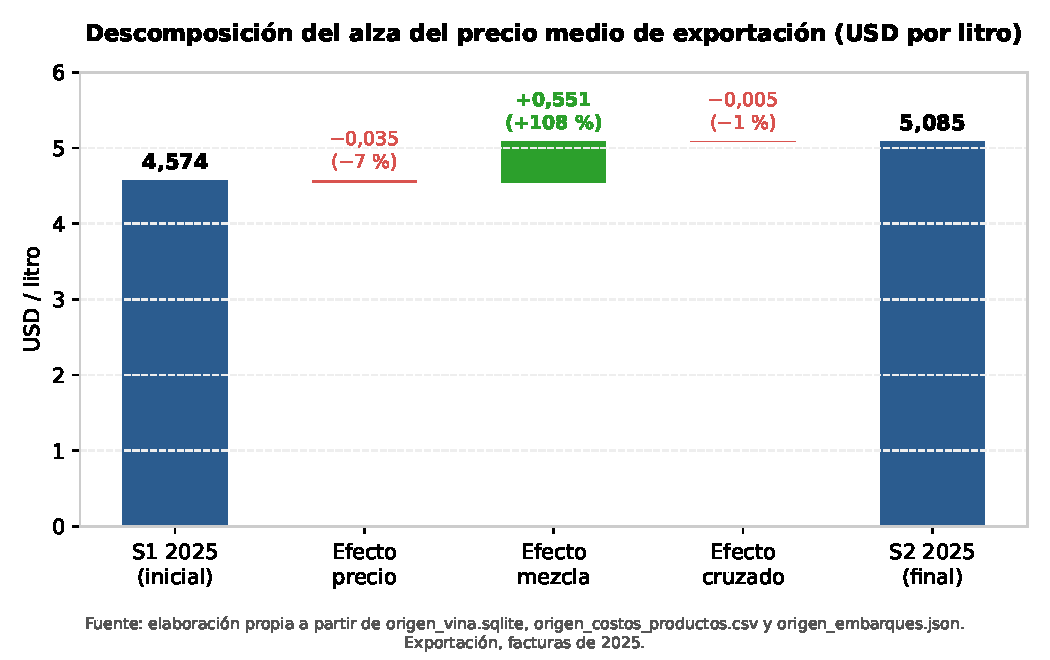
\includegraphics[width=0.44\linewidth]{figura1_cascada_precio.pdf}
  \caption{Descomposición del alza del precio medio de exportación, USD por litro. Fuente: elaboración propia sobre \texttt{fact\_venta} (10.672 líneas de exportación de 2025).}
  \label{fig:cascada}
\end{figure}

\begin{figure}[!htbp]
  \centering
  \begin{minipage}[t]{0.47\textwidth}
    \centering
    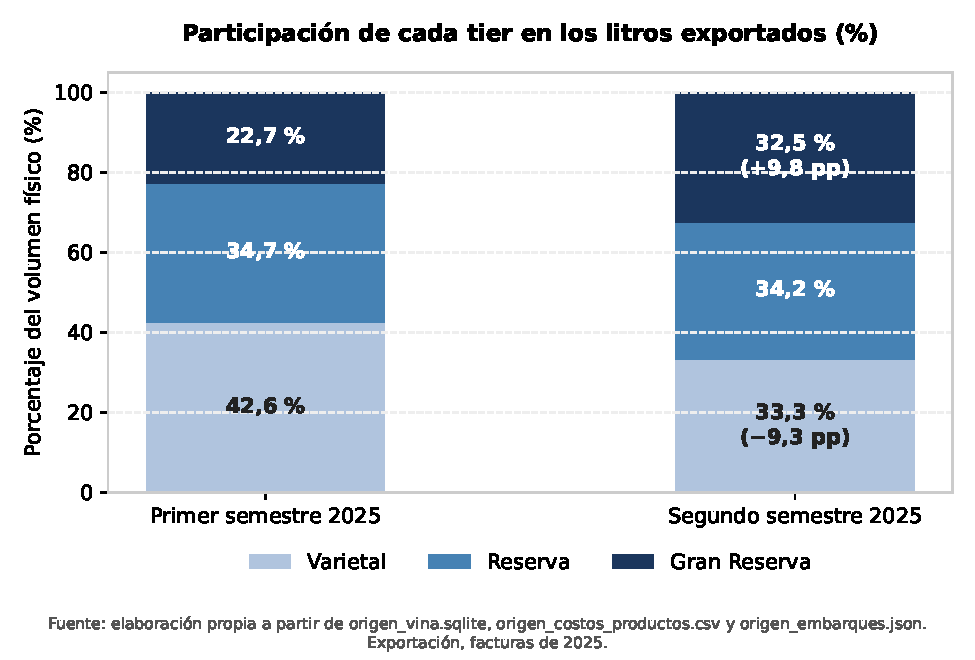
\includegraphics[width=\linewidth]{figura2_mix_semestral.pdf}
    \caption{Participación de cada tier en los litros exportados, \%. Fuente: elaboración propia sobre \texttt{fact\_venta}.}
    \label{fig:mix}
  \end{minipage}\hfill
  \begin{minipage}[t]{0.47\textwidth}
    \centering
    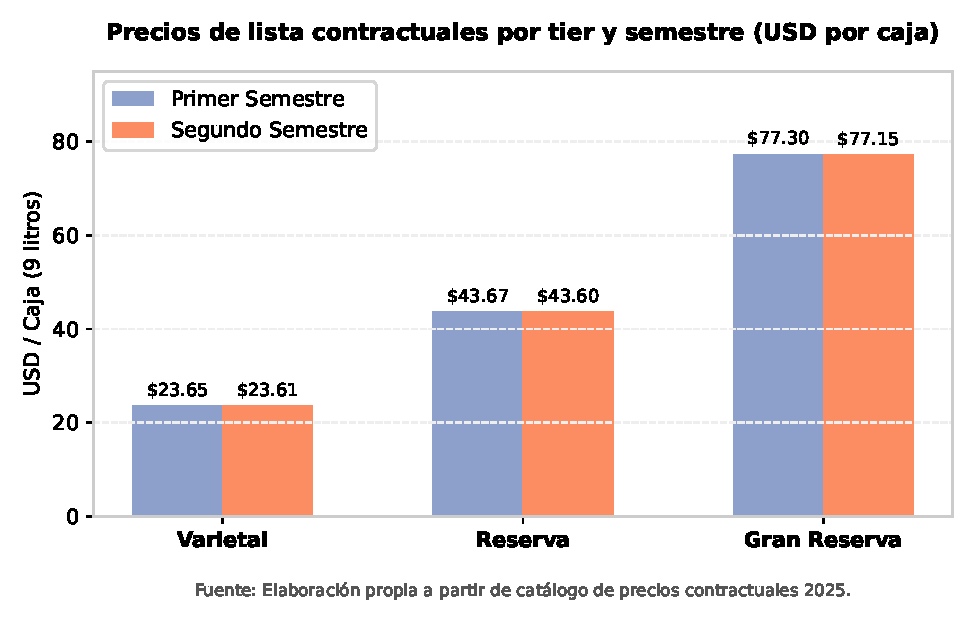
\includegraphics[width=\linewidth]{figura3_precios_lista.pdf}
    \caption{Precio de lista por caja, USD. Fuente: elaboración propia sobre \texttt{fact\_venta}.}
    \label{fig:listas}
  \end{minipage}
\end{figure}

\paragraph{Cuánto vale.} El efecto mezcla aportó 0,551 USD por litro en el 2.\textsuperscript{o} semestre: sobre sus 5.674.554 litros son \textbf{USD 3,13 millones}, o \textbf{CLP 2.961 millones} al tipo de cambio efectivo del semestre (946,34 CLP/USD). Es lo que la viña habría dejado de percibir vendiendo con la mezcla del 1.\textsuperscript{er} semestre, a los mismos precios y volumen.

\paragraph{Y nadie lo está dirigiendo.} Esos CLP 3.000 millones no vienen de una decisión comercial: «no se disgrega cepa, reserva, gran reserva ni varietal al tomar la decisión [\ldots] eso no lo tomamos como una forma de decisión en el día a día» (V). Tampoco es cosa de un cliente: los diez mercados suben entre 7,5 y 12,3 pp de gran reserva (figura~\ref{fig:mercados}, en el anexo). Y el perfil mensual no es el de una temporada: sube sostenidamente de 19,8\,\% en enero a 35,9\,\% en noviembre, y diciembre baja.

\paragraph{Recomendación.} Tres acciones, en orden de lo que cuesta hacerlas:

\begin{enumerate}
\item \textbf{Agregar dos indicadores a la planilla mensual que ya existe.} Comercial descarga el ERP a Excel una vez al mes (V); basta sumar la participación de litros de gran reserva y el precio por litro a mezcla constante. Con eso se distingue mes a mes si la facturación se movió por precio, por descuento o por mezcla, que hoy no se puede separar.
\item \textbf{Fijar la meta en mezcla, no solo en litros.} Finanzas y comercial miran litros totales y operaciones litros por cepa (V), y nadie reconcilia ambas. Una meta explícita de participación por tier alinea la asignación de uva y de bodega con lo que paga el mercado.
\item \textbf{Cerrar la definición de litros por caja en el maestro de productos.} Es una sola columna y de ella cuelga toda la medición por litro (sección~4). Mientras operaciones sostenga que las cajas no rinden lo mismo y el maestro diga 9,0 para ambos formatos, cualquier cifra por litro queda en discusión; el mismo control evita las 151 líneas cargadas este año en botellas en vez de cajas.
\end{enumerate}

\paragraph{Lo que no responde.} Con un solo año no se puede descartar del todo un componente estacional, aunque el patrón observado no es el de una temporada del hemisferio norte (bitácora, S8). El margen por mercado queda fuera: faltan costos de despacho, aranceles y la paridad dólar-euro.

% Sección F · Cobertura de datos. La bitácora y la declaración de IA van en anexos,
% como los pide el enunciado.

\section{Cobertura de datos}

\paragraph{Qué quedó fuera.} De las 13.983 ventas registradas en el ERP quedan fuera \textbf{221, un 1,6\,\%}: 138 duplicados, que sí son un problema de calidad, y 83 facturas de 2026, que quedan en \texttt{fact\_venta} pero fuera del período analizado porque la empresa cierra el año por factura. Por alcance salen además las 3.090 ventas nacionales de 2025. El universo de la métrica son \textbf{10.672 líneas}.

\paragraph{Qué se corrigió sin excluir.} Dentro de ese universo la cadena rectificó 555 montos netos discordantes, 151 líneas cargadas en botellas en vez de cajas, 542 monedas vacías imputadas por mercado y 1.852 costos ausentes imputados por tier y añada (sobre el total registrado, las monedas vacías son 698). Ninguna corrección descarta la transacción: la conserva con la regla aplicada registrada en \texttt{output/cobertura.md}.

\paragraph{Supuestos.} Los trece supuestos que afectan alguna cifra están en el anexo de bitácora, con su justificación y su efecto si fueran falsos. Los que más pesan, S1, S3 y S8, están cuantificados y ninguno invierte la conclusión.


\clearpage
\appendix
% Anexo B · Reglas de limpieza de la cadena. Sale del cuerpo por el límite de 6 páginas.

\section*{Anexo B. Reglas de limpieza de la cadena}
\addcontentsline{toc}{section}{Anexo B. Reglas de limpieza de la cadena}

La cadena no corrige las fuentes: las lee como vienen y aplica reglas explícitas, cada una registrada con su conteo en \texttt{output/cobertura.md}. Las principales: fechas leídas en sus cuatro formatos, 138 duplicados eliminados tras normalizar, precio unitario interpretado según el canal, moneda vacía imputada por mercado, cajas cargadas en botellas divididas por 12 o 10, monto neto recalculado cuando difiere más de 0,5\,\% de cajas $\times$ precio $\times$ (1 $-$ descuento), cepas normalizadas al catálogo del ERP y costos faltantes imputados por tier y añada. Las líneas de merma se conservan; las 83 facturas de 2026 quedan en \texttt{fact\_venta} pero fuera del universo, porque la empresa cierra el año por factura.

Cada regla deja registrado en \texttt{output/cobertura.md} cuántas filas tocó, de modo que la cobertura de la sección~6 se reconstruye desde la ejecución y no a mano.

\clearpage
% Anexo D · Desarrollo de la métrica. Sale del cuerpo por el límite de 6 páginas.

\section*{Anexo D. Métrica: datos de entrada, cálculo y sensibilidades}
\addcontentsline{toc}{section}{Anexo D. Métrica: datos de entrada, cálculo y sensibilidades}

\paragraph{Datos de entrada.} El precio por litro de cada tier, $p_t$, se calcula igual que $P$, pero solo con las ventas de ese tier: la suma de sus $M_i$ dividida por la suma de sus $L_i$. La proporción $w_t$ es la de los litros, no la de las cajas ni la del ingreso.

\begin{center}
\small
\begin{tabular}{l r r r r}
\hline
& \multicolumn{2}{c}{\textbf{Proporción de litros} ($w_t$)} & \multicolumn{2}{c}{\textbf{Precio, USD/L} ($p_t$)} \\
\textbf{Tier} & 1.\textsuperscript{er} sem. & 2.\textsuperscript{o} sem. & 1.\textsuperscript{er} sem. & 2.\textsuperscript{o} sem. \\
\hline
Varietal     & 42,6\,\% & 33,3\,\% & 2,528 & 2,501 \\
Reserva      & 34,7\,\% & 34,2\,\% & 4,659 & 4,643 \\
Gran reserva & 22,7\,\% & 32,5\,\% & 8,277 & 8,197 \\
\hline
\textbf{Total ($P$)} & 100\,\% & 100\,\% & 4,574 & 5,085 \\
\hline
\end{tabular}
\end{center}

\noindent Los tres precios por tier bajaron entre semestres, mientras el precio medio subió. Esa sola observación ya descarta el efecto precio como explicación.

\paragraph{Cálculo.} Aplicando las tres fórmulas tier por tier (en USD/L):

\begin{center}
\small
\begin{tabular}{l r r r}
\hline
& \textbf{Mezcla} & \textbf{Precio} & \textbf{Cruzado} \\
\textbf{Tier} & $(w_{t,2} - w_{t,1})\, p_{t,1}$ & $w_{t,1}\,(p_{t,2} - p_{t,1})$ & $(w_{t,2} - w_{t,1})(p_{t,2} - p_{t,1})$ \\
\hline
Varietal     & $-$0,235 & $-$0,012 & +0,003 \\
Reserva      & $-$0,023 & $-$0,006 & +0,000 \\
Gran reserva & +0,809   & $-$0,018 & $-$0,008 \\
\hline
\textbf{Total} & \textbf{+0,551} & \textbf{$-$0,035} & \textbf{$-$0,005} \\
\hline
\end{tabular}
\end{center}

\noindent Los valores de la tabla están redondeados y el cálculo usa los valores completos (\texttt{output/tablas/fig2\_mezcla\_tier.csv}); por eso la columna de precio suma $-$0,036 en vez de $-$0,035. El efecto mezcla exacto es 0,5515 USD/L, que se publica como 0,551: está a 0,00002 del límite de redondeo, de modo que redondear cualquier valor intermedio antes de multiplicar lo mueve de cifra. Las cantidades derivadas no cambian por eso: 108\,\% del alza, USD 3,13 millones y CLP 2.961 millones.

\paragraph{El efecto precio casi no es precio.} Separando el efecto precio por celda tier $\times$ mercado, solo $-$0,006 USD/L corresponde a cambio de precio dentro de un mismo mercado y tier; $-$0,033 viene de vender más en mercados de menor precio (mezcla de mercados) y $-$0,002 es término cruzado. Las listas prácticamente no se movieron (\texttt{output/tablas/descomposicion\_precio\_mercado.csv}).

\paragraph{Las otras tres decisiones.} Además de los litros por caja, tomamos tres decisiones al construir la métrica. Para cada una repetimos el análisis completo con la opción que no elegimos:

\begin{center}
\small
\begin{tabular}{p{2.6cm} p{4.3cm} p{4.3cm} r}
\hline
\textbf{Decisión} & \textbf{Lo que usamos} & \textbf{Alternativa probada} & \textbf{Mezcla, \% del alza} \\
\hline
Método de descomposición & Base en el 1.\textsuperscript{er} semestre, con el término cruzado aparte (107,9\,\%) & Los otros tres métodos usuales: simétrico, que reparte el cruzado por mitades, y dos secuenciales, que se lo asignan entero a la mezcla o al precio & 106,9 a 107,9\,\% \\[2pt]
Líneas de merma & Incluidas: las cajas descartadas por merma restan litros e ingreso (107,9\,\%) & Excluidas: se ignoran esas líneas & 108,0\,\% \\[2pt]
Precio usado & Neto: lo que el cliente pagó, después de descuento (107,9\,\%) & De lista: antes de descuento & 101,7\,\% \\
\hline
\end{tabular}
\end{center}

\noindent Con el precio de lista la mezcla explica algo menos (101,7\,\%) porque desaparece el aumento del descuento, que restaba al efecto precio; aun así sigue sobre el 100\,\%. El detalle de las cinco sensibilidades está en \texttt{output/tablas/sensibilidades.csv}.

\paragraph{Medición en pesos.} Los contratos se firman en dólares (V), y medir en esa moneda aísla el precio y la mezcla del tipo de cambio. En pesos el alza es menor: 10,1\,\% convirtiendo con el dólar observado de la fecha de factura y 6,3\,\% con el de la fecha estimada de cobranza (factura más 60 días para el hemisferio sur y 90 para el norte, según la contraparte), contra 11,2\,\% en dólares. Esa diferencia es efecto del tipo de cambio, que no es ni precio ni mezcla, de modo que la descomposición en pesos no es comparable con la de dólares.

\clearpage
% Anexo de la sección C. Requiere en el preámbulo: array, booktabs, longtable.

\section*{Anexo C. Modelo dimensional: matrices y diccionario de datos}

\subsection*{C.1 Matriz de hechos y calificadores}

Incluye las cuatro preguntas del README y las dos que la contraparte planteó en la reunión del 4 de septiembre. En cada una, el verbo de medición es el hecho y cada ``por'' es un calificador.

\begin{center}
\small
\begin{tabular}{@{}>{\raggedright\arraybackslash}p{0.40\textwidth}>{\raggedright\arraybackslash}p{0.25\textwidth}>{\raggedright\arraybackslash}p{0.28\textwidth}@{}}
\toprule
Pregunta del negocio & Hecho (qué se mide) & Calificadores (por dónde se corta) \\
\midrule
¿El precio por litro subió por precio o por mezcla? (README 2, la elegida) & Monto neto, litros & Tier, semestre, mercado \\
¿Las exportaciones crecen en pesos? (README 1) & Monto neto en dólares y pesos, tipo de cambio & Mes, semestre, mercado \\
¿Qué mercados crecieron en volumen y con qué margen? (README 3) & Litros, monto neto, costo total & Mercado, semestre, tier \\
¿Qué fecha usar para convertir y qué ingreso comparar con el costo? (README 4) & Monto neto, costo total, tipo de cambio & Fecha de factura, fecha de embarque \\
¿Cuántos litros vendemos de cada cepa y de cada tier? (reunión) & Litros & Cepa, tier, mercado, mes \\
¿En qué mercados poner más esfuerzo? (reunión) & Litros, monto neto & Mercado, cliente, tier \\
\bottomrule
\end{tabular}
\end{center}

Lo que revela la matriz: el monto neto y los litros se repiten en casi todas las preguntas, así que comparten grano y van en la misma tabla de hechos. Tiempo, mercado y producto (tier y cepa) aparecen en varias preguntas: son las dimensiones conformadas. La fecha de embarque pertenece a otro proceso, el embarque, y por eso no entra a esta estrella.

\subsection*{C.2 Matriz de bus}

\begin{center}
\small
\begin{tabular}{@{}lccccc@{}}
\toprule
Proceso & Tiempo & Producto & Cliente & Mercado & Incoterm \\
\midrule
Venta (modelada en la Entrega 1) & $\bullet$ & $\bullet$ & $\bullet$ & $\bullet$ & \\
Embarque (candidato, JSON) & $\bullet$ & $\bullet$ & & $\bullet$ & $\bullet$ \\
Cobranza (candidato, sin fechas de pago) & $\bullet$ & & $\bullet$ & $\bullet$ & \\
\bottomrule
\end{tabular}
\end{center}

Tiempo y mercado se repiten en los tres procesos: si cada área los definiera distinto, ningún cruce entre venta, embarque y cobranza cuadraría. Por eso se definen una sola vez.

\subsection*{C.3 Dimensiones que cambian}

Las fuentes son una foto sin historia de cambios, así que todas las dimensiones se cargan con tipo 1 (sobrescribir). Si en adelante el maestro de productos cambiara el costo o los litros por caja de un producto, habría que versionar ese atributo (tipo 2), para que las ventas pasadas conserven el valor vigente al momento de la venta.

\subsection*{C.4 Diccionario de datos}

% Generado por src/generar_diccionario.py desde src/esquema.py. No editar a mano.

\subsubsection*{\texttt{fact\_venta}}
Hecho transaccional. Una fila por línea de venta facturada.

{\footnotesize
\begin{longtable}{@{}>{\raggedright\arraybackslash}p{0.19\textwidth}>{\raggedright\arraybackslash}p{0.1\textwidth}>{\raggedright\arraybackslash}p{0.085\textwidth}>{\raggedright\arraybackslash}p{0.205\textwidth}>{\raggedright\arraybackslash}p{0.27\textwidth}@{}}
\toprule
Columna & Rol & Aditiv. & Descripción & Origen y regla \\
\midrule
\endhead
\texttt{venta\_id} & degenerada & — & Número de la línea en el ERP. & ventas.\allowbreak{}venta\_id; deduplicado tras normalizar formatos \\
\texttt{fecha\_key} & llave & — & Fecha de factura. & ventas.\allowbreak{}fecha, leída en sus 4 formatos \\
\texttt{producto\_anada\_key} & llave & — & Producto y añada vendidos. & ventas.\allowbreak{}producto\_id + ventas.\allowbreak{}anada \\
\texttt{cliente\_key} & llave & — & Cliente que compra. & ventas.\allowbreak{}cliente\_id \\
\texttt{mercado\_key} & llave & — & Mercado de destino. & ventas.\allowbreak{}mercado\_id (coincide con clientes.\allowbreak{}mercado\_id) \\
\texttt{cajas} & medida & aditiva & Cajas vendidas; negativas si la línea es merma. & ventas.\allowbreak{}cajas; si vienen en botellas (12 o 10 veces las cajas del embarque), se dividen por el factor \\
\texttt{litros} & medida & aditiva & Litros vendidos. & cajas $\times$ dim\_producto.\allowbreak{}litros\_por\_caja \\
\texttt{monto\_bruto\_clp} & medida & aditiva & Monto antes de descuento, en pesos. & cajas $\times$ precio unitario; si la moneda es USD, $\times$ tipo\_cambio \\
\texttt{monto\_bruto\_usd} & medida & aditiva & Monto antes de descuento, en dólares. & cajas $\times$ precio unitario; si la moneda es CLP, $\div$ tipo\_cambio \\
\texttt{monto\_neto\_clp} & medida & aditiva & Ingreso neto de descuento, en pesos. & cajas $\times$ precio unitario $\times$ (1 $-$ descuento), convertido con tipo\_cambio \\
\texttt{monto\_neto\_usd} & medida & aditiva & Ingreso neto de descuento, en dólares. & cajas $\times$ precio unitario $\times$ (1 $-$ descuento), convertido con tipo\_cambio \\
\texttt{costo\_total\_clp} & medida & aditiva & Costo de producción de lo vendido, en pesos. & \textbar{}cajas\textbar{} $\times$ dim\_producto.\allowbreak{}costo\_caja\_clp; en la merma el costo no se reversa \\
\texttt{tipo\_cambio} & contexto & no aditiva & Dólar observado usado para convertir la línea. & API mindicador.\allowbreak{}cl, fecha de factura; fines de semana y feriados con el último día hábil previo \\
\texttt{es\_merma} & indicador & aditiva & 1 si la línea es merma (cajas negativas). & cajas < 0; merma según la contraparte (4 sep) \\
\texttt{monto\_recalculado} & indicador & aditiva & 1 si el monto registrado no cuadraba y se recalculó. & \textbar{}monto registrado $-$ calculado\textbar{} > 0,5 \% \\
\texttt{cajas\_corregidas} & indicador & aditiva & 1 si las cajas venían en botellas. & cruce con origen\_embarques.\allowbreak{}json \\
\texttt{moneda\_imputada} & indicador & aditiva & 1 si la moneda venía vacía. & ventas.\allowbreak{}moneda\_id nulo; se imputa por mercado \\
\bottomrule
\end{longtable}
}

\subsubsection*{\texttt{dim\_tiempo}}
Una fila por día calendario de 2025.

{\footnotesize
\begin{longtable}{@{}>{\raggedright\arraybackslash}p{0.19\textwidth}>{\raggedright\arraybackslash}p{0.1\textwidth}>{\raggedright\arraybackslash}p{0.085\textwidth}>{\raggedright\arraybackslash}p{0.205\textwidth}>{\raggedright\arraybackslash}p{0.27\textwidth}@{}}
\toprule
Columna & Rol & Aditiv. & Descripción & Origen y regla \\
\midrule
\endhead
\texttt{fecha\_key} & llave & — & Llave AAAAMMDD. & generada \\
\texttt{fecha} & atributo & — & Fecha. & calendario \\
\texttt{dia\_semana} & atributo & — & Lunes a domingo. & calendario \\
\texttt{semana} & atributo & — & Semana del año. & calendario \\
\texttt{mes} & atributo & — & Mes (número y nombre). & calendario \\
\texttt{trimestre} & atributo & — & Trimestre. & calendario \\
\texttt{semestre} & atributo & — & Primer o segundo semestre. & calendario \\
\texttt{anio} & atributo & — & Año. & calendario \\
\texttt{es\_dia\_habil} & atributo & — & 1 si es día hábil. & 1 si la API del dólar publica valor ese día \\
\texttt{es\_feriado} & atributo & — & 1 si es feriado. & día de semana sin valor publicado en la API \\
\bottomrule
\end{longtable}
}

\subsubsection*{\texttt{dim\_producto}}
Una fila por producto y añada (24 productos $\times$ 4 añadas = 96 filas).

{\footnotesize
\begin{longtable}{@{}>{\raggedright\arraybackslash}p{0.19\textwidth}>{\raggedright\arraybackslash}p{0.1\textwidth}>{\raggedright\arraybackslash}p{0.085\textwidth}>{\raggedright\arraybackslash}p{0.205\textwidth}>{\raggedright\arraybackslash}p{0.27\textwidth}@{}}
\toprule
Columna & Rol & Aditiv. & Descripción & Origen y regla \\
\midrule
\endhead
\texttt{producto\_anada\_key} & llave & — & Llave producto-añada. & generada \\
\texttt{producto} & atributo & — & Nombre del vino. & origen\_costos\_productos.\allowbreak{}csv: producto \\
\texttt{cepa} & atributo & — & Cepa, con el nombre oficial del catálogo del ERP. & CSV: cepa, normalizada desde sus alias y conformada a origen\_vina.\allowbreak{}sqlite: cepas.\allowbreak{}cepa; desempate en la bitácora \\
\texttt{tipo\_vino} & atributo & — & Tinto o blanco. & origen\_vina.\allowbreak{}sqlite: cepas.\allowbreak{}tipo \\
\texttt{tier} & atributo & — & Varietal, Reserva o Gran Reserva. & CSV: tier \\
\texttt{formato} & atributo & — & 12 $\times$ 750 ml o 6 $\times$ 1500 ml. & CSV: formato \\
\texttt{litros\_por\_caja} & atributo & — & Litros que rinde una caja: la definición de caja a litro. & CSV: litros\_por\_caja (9,0 para ambos formatos) \\
\texttt{anada} & atributo & — & Año de cosecha. & CSV: anada \\
\texttt{costo\_caja\_clp} & atributo & — & Costo unitario de producción por caja. & CSV: costo\_caja\_clp; si falta, regla exacta (tier, añada) \\
\texttt{costo\_imputado} & atributo & — & 1 si el costo se imputó por regla. & generado \\
\texttt{activo} & atributo & — & Si el producto sigue en catálogo. & CSV: activo (si/SI/Sí/1 = verdadero) \\
\bottomrule
\end{longtable}
}

\subsubsection*{\texttt{dim\_cliente}}
Una fila por cliente (distribuidor o importador).

{\footnotesize
\begin{longtable}{@{}>{\raggedright\arraybackslash}p{0.19\textwidth}>{\raggedright\arraybackslash}p{0.1\textwidth}>{\raggedright\arraybackslash}p{0.085\textwidth}>{\raggedright\arraybackslash}p{0.205\textwidth}>{\raggedright\arraybackslash}p{0.27\textwidth}@{}}
\toprule
Columna & Rol & Aditiv. & Descripción & Origen y regla \\
\midrule
\endhead
\texttt{cliente\_key} & llave & — & Llave del cliente. & generada \\
\texttt{cliente\_id} & atributo & — & Código del ERP. & origen\_vina.\allowbreak{}sqlite: clientes.\allowbreak{}cliente\_id \\
\texttt{nombre} & atributo & — & Razón social. & clientes.\allowbreak{}nombre \\
\texttt{tipo} & atributo & — & Distribuidor o importador. & clientes.\allowbreak{}tipo \\
\bottomrule
\end{longtable}
}

\subsubsection*{\texttt{dim\_mercado}}
Una fila por mercado de destino. País y zona son niveles de una misma jerarquía.

{\footnotesize
\begin{longtable}{@{}>{\raggedright\arraybackslash}p{0.19\textwidth}>{\raggedright\arraybackslash}p{0.1\textwidth}>{\raggedright\arraybackslash}p{0.085\textwidth}>{\raggedright\arraybackslash}p{0.205\textwidth}>{\raggedright\arraybackslash}p{0.27\textwidth}@{}}
\toprule
Columna & Rol & Aditiv. & Descripción & Origen y regla \\
\midrule
\endhead
\texttt{mercado\_key} & llave & — & Llave del mercado. & generada \\
\texttt{pais} & atributo & — & País de destino. & origen\_vina.\allowbreak{}sqlite: mercados.\allowbreak{}pais \\
\texttt{zona} & atributo & — & Zona comercial. & mercados.\allowbreak{}zona\_id $\rightarrow$ zonas.\allowbreak{}zona; zona 8 inexistente (Corea del Sur) se asigna a Asia \\
\texttt{canal} & atributo & — & Nacional o Exportación. & mercados.\allowbreak{}canal \\
\texttt{hemisferio} & atributo & — & Norte o sur. & derivado del país (Chile y Brasil: sur) \\
\texttt{moneda\_facturacion} & atributo & — & CLP o USD. & monedas.\allowbreak{}moneda; en los datos la moneda queda determinada por el mercado (Chile CLP, resto USD); el ETL verifica que no haya excepciones \\
\bottomrule
\end{longtable}
}


\clearpage
% Anexo · Bitácora de supuestos. Cifras verificadas contra output/cifras.md.

\section*{Anexo. Bitácora de supuestos}
\addcontentsline{toc}{section}{Anexo. Bitácora de supuestos}

Origen de cada hallazgo: \textbf{(V)} verbalizado por la contraparte, \textbf{(M)} medido sobre los datos, \textbf{(I)} inferido por el equipo. Las consultas enviadas por el hilo de correo no fueron respondidas, de modo que los supuestos quedan cerrados con criterio propio y cuantificados.

\begin{longtable}{p{0.6cm} p{3.0cm} c p{4.3cm} p{4.3cm} p{2.0cm}}
\toprule
\textbf{ID} & \textbf{Supuesto} & \textbf{Origen} & \textbf{Justificación} & \textbf{Efecto si fuera falso} & \textbf{Decisión} \\
\midrule
\endhead

\textbf{S1} & Una caja rinde 9,0\,L en los dos formatos (12$\times$750\,ml y 6$\times$1500\,ml). & M/I & El maestro de costos lo declara para ambos (M) y la aritmética de los formatos da 9\,L exactos. El precio de lista por caja coincide entre magnum y gran reserva estándar (77,26 y 77,20 USD) y el costo por caja es idéntico (M), lo que solo se sostiene si rinden lo mismo (I). & Con 18\,L el precio medio anual sería 4,47 USD/L ($-$7,5\,\%); con 4,5\,L, 5,03 (+4,2\,\%). La mezcla sigue explicando 108\,\% del alza en los tres casos: la conclusión no cambia. & Equipo, 4 sep \\
\midrule
\textbf{S2} & Las cajas cargadas como botellas se dividen por 12 o por 10. & M & 151 líneas cuyo total no cuadra con el embarque de la misma venta; el factor se identifica contra \texttt{origen\_embarques.json} (M). & Sin corregir, los litros se sobreestiman y el precio por litro baja artificialmente en esas líneas. & Equipo, sep \\
\midrule
\textbf{S3} & El monto neto se recalcula como cajas $\times$ precio $\times$ (1 $-$ descuento) cuando el registrado difiere más de 0,5\,\%. & V/M & El 94,5\,\% de las filas cuadra con esa fórmula a $\pm$0,5\,\% (M), así que la fórmula es la regla y el resto es ruido de carga. La gerencia declaró que «en esta empresa no se pierde ni un peso» (V). & Si el monto registrado fuera el real (por ejemplo, rebates no declarados), el ingreso de exportación cambiaría en CLP 2.096 millones. & Equipo, sep \\
\midrule
\textbf{S4} & La moneda vacía se imputa por mercado: Chile en CLP, el resto en USD. & M & 698 registros sin moneda (5,0\,\%), repartidos de forma pareja por mercado, vendedor, mes y cliente: no hay patrón de negocio, es pérdida de campo en la carga (M). Los rangos de precio separan ambas monedas sin ambigüedad (20.428--72.290 en CLP, 22--80 en USD). & Filas convertidas con la moneda equivocada: error de escala de tres órdenes de magnitud. & Equipo, sep \\
\midrule
\textbf{S5} & Los costos ausentes se imputan por tier y añada. & M & Las 81 filas del maestro siguen una regla determinista por tier y añada, sin una sola excepción (M). Faltan 15 pares de la añada 2021 y un valor \texttt{N/A}. & No afecta el precio por litro ni la facturación; cambiaría el margen bruto en el 17,4\,\% de las filas del universo. & Equipo, sep \\
\midrule
\textbf{S6} & Los montos se convierten a pesos con el dólar observado de la fecha de factura. & V/I & Finanzas no tiene política formal de tipo de cambio (V), pero sí declaró que el año «se cierra por factura, no por despacho» (V); adoptamos la misma fecha por consistencia (I). & El ingreso en pesos varía $-$0,91\,\% a fecha de embarque y $-$2,14\,\% a fecha de cobranza (60 días hemisferio sur, 90 norte). No afecta la métrica, que está en USD/L. & Contraparte (cierre) y equipo (conversión), 4 sep \\
\midrule
\textbf{S7} & Las líneas negativas son merma: restan litros e ingreso, pero su costo no se reversa. & V/I & «Si se pierde la cadena de frío se descartan esas cajas; es considerado dentro de la merma» (V). El vino se produjo y se perdió, así que el costo ya se devengó (I). & Reversar el costo subiría el margen bruto de 47,25\,\% a 48,05\,\%, una diferencia de CLP 419 millones. & Contraparte y equipo, 4 sep \\
\midrule
\textbf{S8} & La comparación entre semestres mide un cambio de mezcla estructural y no solo estacionalidad. & M/I & Es el supuesto más expuesto, porque solo hay un año de datos y la contraparte declaró que la venta es contracíclica al hemisferio norte con «fuerte estacionalidad en el cambio de estación» (V). Tres mediciones apuntan en contra de esa explicación (M): \textbf{(a)} Brasil, el único mercado de exportación del hemisferio sur, sube de 22,7\,\% a 31,5\,\% de gran reserva, igual que los del norte; una estacionalidad de fin de año del hemisferio norte no debería aparecer ahí. \textbf{(b)} La participación mensual sube de forma sostenida, de 19,8\,\% en enero a 35,9\,\% en noviembre, y diciembre baja a 35,2\,\%: no tiene forma de peak de temporada. \textbf{(c)} Los diez mercados suben entre 7,5 y 12,3 pp, así que no es un cliente ni una región. & Con un año no se puede descartar del todo un componente estacional (I). Si el alza fuera puramente cíclica, la premiumización se revertiría en el 1.\textsuperscript{er} semestre de 2026 y la recomendación pasaría de dirigir la mezcla a planificar stock estacional. La magnitud del efecto en 2025 (CLP 2.961 millones) no cambia. & Equipo, oct \\
\midrule
\textbf{S9} & La mezcla se descompone a nivel de tier (tres categorías). & V/I & Es el nivel que la contraparte nombró como el que no disgrega al decidir (V) y el que separa los precios por litro sin solapamiento: 2,5, 4,7 y 8,3 USD/L (M). & Descomponer por los 24 productos reparte el efecto en más celdas, pero no cambia el signo ni el orden de magnitud de la mezcla. & Equipo, sep \\
\midrule
\textbf{S10} & El dólar observado representa el tipo de cambio efectivamente liquidado. & I & La contraparte no mencionó cobertura cambiaria en toda la reunión, ni al preguntarle por el tipo de cambio (V); asumimos que no la hay (I). & Con forwards, el ingreso en pesos sería distinto del que calculamos. No afecta la métrica en USD/L ni la descomposición. & Equipo, sep \\
\midrule
\textbf{S11} & El tramo cambiario dólar-euro queda fuera del modelo. & V/M & «Todos los contratos se hacen en dólares, pero los clientes europeos pagan en euros» (V). No hay paridad USD/EUR en ninguna de las cuatro fuentes (M). & Afecta al 32\,\% del ingreso de exportación (Alemania, Países Bajos y Reino Unido) al convertir a pesos, pero no el valor facturado en dólares. & Contraparte y equipo, 4 sep \\
\midrule
\textbf{S12} & Las fechas ambiguas \texttt{dd/mm/aaaa} se leen como día/mes. & M & Es el formato declarado de los otros tres patrones de fecha del mismo campo (M). La columna \texttt{mes} del ERP no sirve para dirimirlo: discrepa de la fecha en 981 filas, también en fechas ISO sin ambigüedad (M). & 1.387 fechas admiten las dos lecturas; 121 de ellas calzarían con la columna \texttt{mes} leídas como mes/día. Leerlas al revés movería de mes a lo más esas 121 líneas, sin efecto en la agregación semestral salvo las que cruzan junio o diciembre. & Equipo, sep \\
\midrule
\textbf{S13} & El mercado de Corea del Sur, con \texttt{zona\_id} 8 inexistente, se asigna a Asia. & I & La tabla de zonas llega hasta 5 y los demás mercados asiáticos están en Asia (M). & Sin corregir, 1.059 líneas quedan sin zona y Asia queda subrepresentada en los cortes por región. & Equipo, sep \\
\bottomrule
\end{longtable}

\begin{figure}[!htbp]
  \centering
  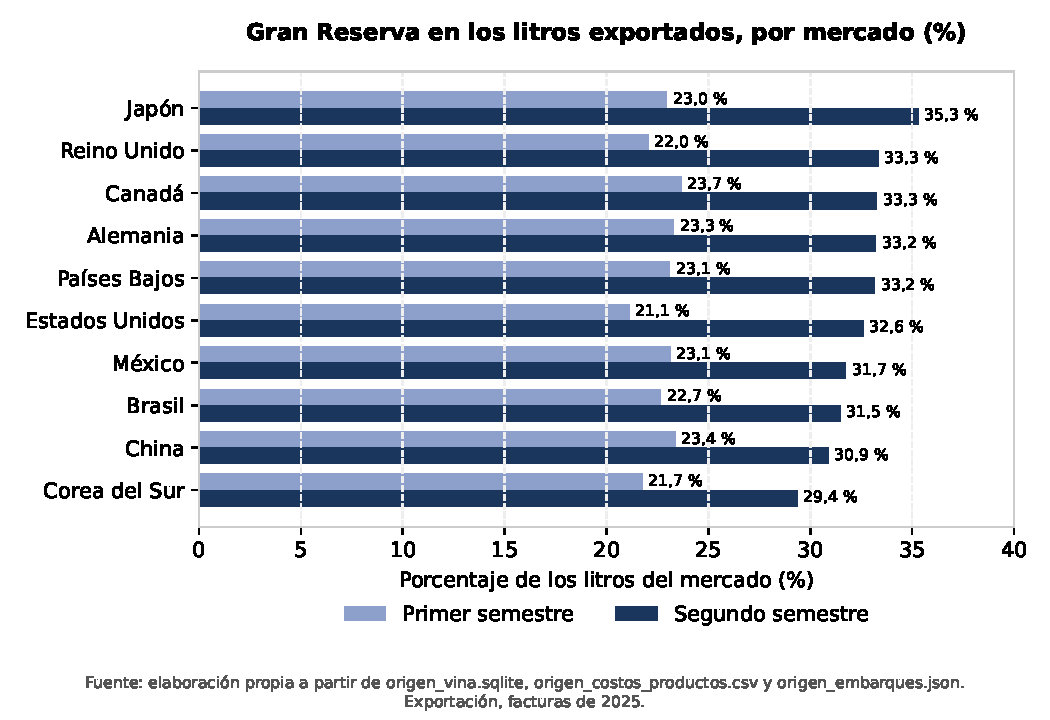
\includegraphics[width=0.58\linewidth]{figura4_gran_reserva_mercados.pdf}
  \caption{Participación de gran reserva en los litros, por mercado y semestre, \%. Fuente: elaboración propia sobre \texttt{fact\_venta}.}
  \label{fig:mercados}
\end{figure}

\noindent La figura respalda el supuesto S8: los diez mercados de exportación suben su participación de gran reserva entre el 1.\textsuperscript{er} y el 2.\textsuperscript{o} semestre, entre 7,5 pp (China) y 12,3 pp (Japón). Brasil, el único del hemisferio sur, sube 8,8 pp.

\clearpage
% Anexo · Declaración de uso de IA. El enunciado la pide como anexo obligatorio.

\section*{Anexo. Declaración de uso de inteligencia artificial}
\addcontentsline{toc}{section}{Anexo. Declaración de uso de inteligencia artificial}

Se usaron Claude (Anthropic) y Gemini (Google) como apoyo en la exploración inicial de las fuentes, en la escritura del código de la cadena de datos, en la redacción y edición del informe y en la revisión de sintaxis LaTeX. Las decisiones de alcance, las definiciones de la métrica y los supuestos de la bitácora los tomó el equipo. Todas las cifras del informe se generan con \texttt{python run.py} y quedan contrastadas contra los datos en \texttt{output/cifras.md}.


\end{document}
